\subsection{Validation and Testing Procedures for Model Evaluation}\label{subsec:validation_testing_procedures}
This section describes the validation and testing procedures our experiments follow.
Selecting appropriate testing procedures is crucial for ensuring the validity and reliability of the results.
For that reason, we delineate a methodological approach that ensures our models are accurate and generalizable.
We begin by outlining our general strategy for model evaluation.
Next, we describe the procedure used to partition our dataset into training, validation, and testing sets.
Finally, we present the evaluation metrics used to assess the performance of our models.

We have chosen to test and evaluate all our experiments using both cross-validation and a separate test set.
Evaluating results solely on the test set could lead to models that are overly specialized to the test set.
This occurs when searching for the optimal configuration of hyperparameters specifically tailored to the test set.
For this reason, it is common to use a validation set to tune hyperparameters and evaluate model performance during experimentation.
However, further splitting the training set into a validation set exacerbates the challenges of limited data availability, as described in Section~\ref{subsec:challenges}.
Our objective is to develop models that demonstrate high accuracy and robustness, even on entirely unseen data.
To achieve this, we employ $k$-fold cross-validation.
This allows us to train our models on $k-1$ folds and evaluate them on the remaining fold, which provides a more robust estimate of model performance, and allows us to use all the data for training.
Since our approach includes large-scale optimization, we prefer $k$-fold cross-validation over \gls{loocv}.
\gls{loocv} uses each individual sample as a single test case, resulting in $n$ iterations, where $n$ is the number of samples.
In each iteration, models and preprocessors would need to be refit, making this approach too computationally expensive and time-consuming for the scope of our study.

While we employ conventional techniques like holdout sets and k-fold cross validation, the dataset we use imposes additional challenges to the process.

One of the primary challenges is preventing data leakage.
As per concentration matrix $\mathbf{C}$ in Section~\ref{sec:problem_definition}, each target only has one ground truth concentration value per oxide.
However, each target is shot at multiple locations, resulting in multiple instances of the same target in the dataset, as shown in Table~\ref{tab:final_dataset_example}.
Although the intensity values vary for each location, they fundamentally represent measurements of the same target.
If we were to randomly split the dataset, some locations from a target could end up in the testing set while others remain in the training set.
This would cause data leakage, as the testing set would no longer consist solely of unseen targets.
To prevent this, we ensure that each target is represented only once in the dataset by grouping data from all locations on a given target.

Furthermore, the limited availability of data poses another significant challenge.
The dataset we use consists of 408 samples, which is relatively large by \gls{libs} standards.
However, there are only a few samples with concentration values for the oxides in the targets that are either very high or very low compared to the rest of the data, which we refer to as \textit{extreme values}.
These infrequent high and low concentration values can be problematic.
If such values end up in the test set, the model may be evaluated on data points outside the range it was trained on.
This situation can lead to an inaccurate assessment of the model's performance, as it might not handle these uncommon concentration ranges effectively.

When performing a random split of the dataset into multiple folds for cross-validation, as well as for training and testing sets, this small number of extreme values can result in an uneven distribution.
The presence or absence of these extreme values in any given fold can heavily influence the model's performance metrics.
If extreme values are disproportionately allocated to the testing set, the resulting model may struggle to generalize accurately.
This uneven distribution can lead to models that perform well on the majority of the data but fail to predict accurately for these extreme concentration values.
Conversely, if the scarce extreme values are disproportionately assigned to the training set, the model may become overly specialized in handling these extreme values, potentially leading to overfitting.
This means the model might perform well on the training set, including the extreme values, but fail to generalize effectively to new, unseen data, especially if the test set does not contain similar extreme values.
This could result in an inaccurate assessment of the model's performance, as the test set would not adequately challenge the model's ability to predict across the full range of data variability.

\begin{figure*}[h!]
    \centering
    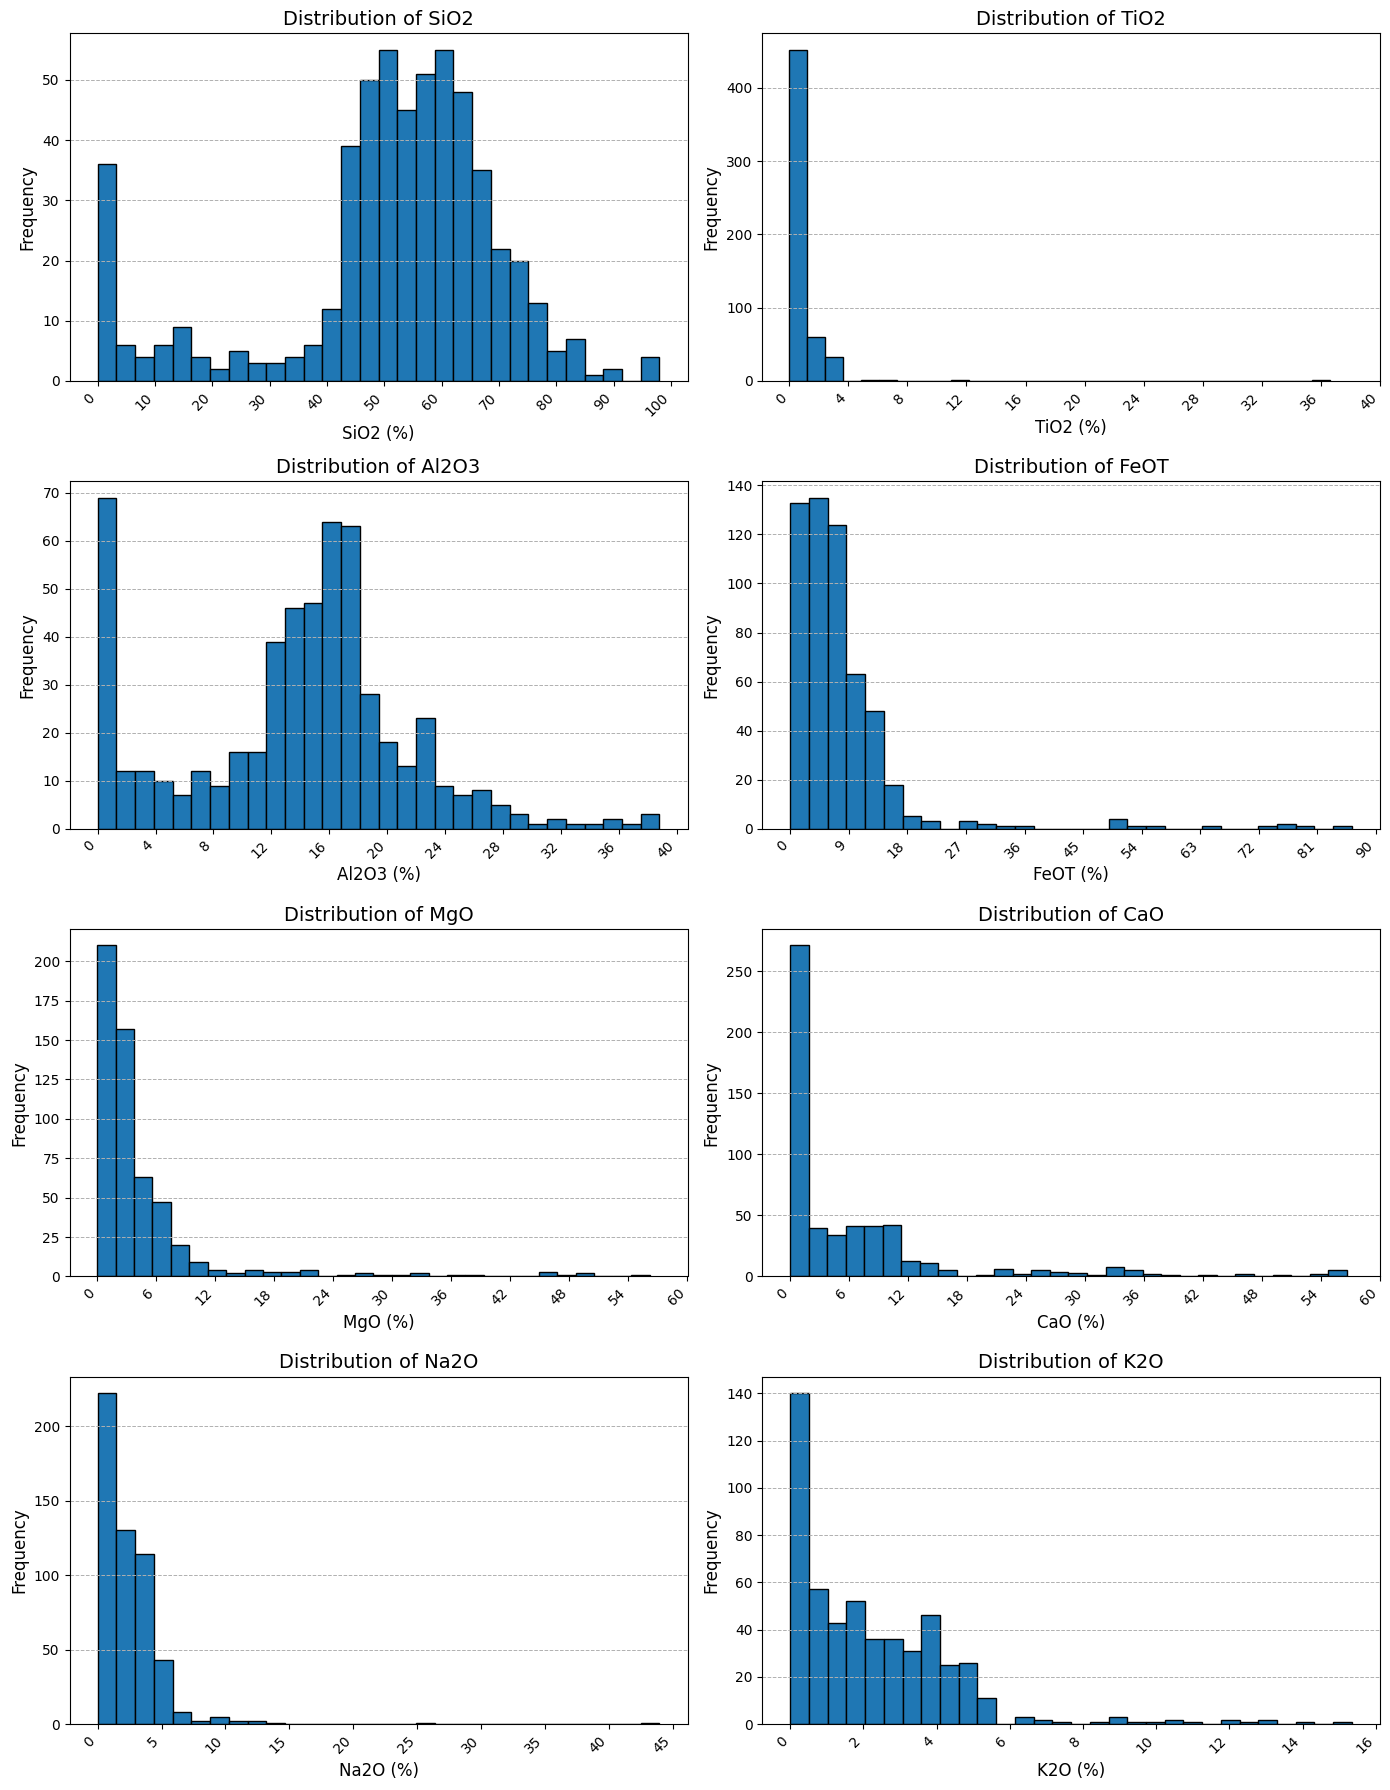
\includegraphics[width=\textwidth]{images/oxide_distributions.png}
    \caption{Distributions of various oxide concentrations in the dataset. The histograms show the frequency of concentration values for \ce{SiO2}, \ce{TiO2}, \ce{Al2O3}, \ce{FeO_T}, \ce{MgO}, \ce{CaO}, \ce{Na2O}, and \ce{K2O}.}
    \label{fig:oxide_distributions}
\end{figure*}

Figure~\ref{fig:oxide_distributions} illustrates the distributions of various oxide concentrations in our dataset.
Across all oxides, there is a general pattern of skewed distributions, with concentrations heavily weighted towards lower values.
This is particularly notable in \ce{TiO2}, \ce{FeO_T}, \ce{MgO}, \ce{CaO}, and \ce{Na2O}.
\ce{SiO2} and \ce{Al2O3} show more variability, with \ce{SiO2} exhibiting a bimodal distribution.
These distributions confirm the presence of extreme values across all oxides, which are significantly overrepresented or underrepresented, further complicating the model training process.

This necessitates careful dataset partitioning to ensure that the model training process accounts for these challenges, improving the generalizability and robustness of the models.

\subsubsection{Dataset Partitioning}\label{subsubsec:dataset_partitioning}
To ensure rigorous evaluation of our models and to address the challenges of data leakage and uneven distribution of extreme values, we have implemented a customized k-fold data partitioning procedure. 
This approach divides the dataset into $k$ folds, which are used to define cross-validation datasets, as well as a training set and a test set.
The procedure ensures that all data points from a given target are only present in one of the $k$ folds, effectively preventing the aforementioned data leakage.
Additionally, it ensures that extreme values are handled by redistributing them evenly across the training folds, preventing any single fold from being disproportionately influenced by these values.

\begin{algorithm}
\caption{Data Partitioning With Extreme Value Handling}
\label{alg:custom_kfold_cv}
\begin{algorithmic}[1]
\Require Dataset $\mathbf{D}$, group column $g$, target column $t$, number of splits $k$, percentile $p$, random seed $\textit{seed}$
\Ensure Training and validation sets for cross-validation $\mathbf{T}_\text{cv}$, training set $\mathbf{D}_\text{train}$, and test set $\mathbf{D}_\text{test}$
\State \label{line:seed} Set random seed for reproducibility if $\text{seed}$ is not None
\State \label{line:remove_duplicates} Remove duplicate entries based on $g$ and sort by $t$
\State \label{line:assign_folds} Assign fold numbers sequentially from 0 to $k-1$ to unique targets
\If{extreme values handling is enabled}
    \State \label{line:identify_extremes} Identify extreme values at percentiles $p$ and $1-p$
    \State \label{line:reassign_extremes} Reassign extreme values to folds $0$ to $k-2$
\EndIf
\State \label{line:merge_folds} Merge fold assignments information into the original dataset
\State \label{line:split_dataset} Split dataset into test set $\mathbf{D}_\text{test}$ (fold $k-1$) and remaining data $\mathbf{D}_\text{train}$
\State \label{line:create_folds} Create $k-1$ training and validation sets
\For{each fold $i$ from 0 to $k-2$}
    \State $\mathbf{T}_\text{train}[i] \gets \mathbf{D}_\text{train} \setminus \text{fold}_i$
    \State $\mathbf{T}_\text{val}[i] \gets \text{fold}_i$
    \State Append $(\mathbf{T}_\text{train}[i], \mathbf{T}_\text{val}[i])$ to $\mathbf{T}_\text{cv}$
\EndFor
\State \label{line:remove_fold_column} Remove fold column from all datasets
\State \Return $\mathbf{T}_\text{cv}, \mathbf{D}_\text{train}, \mathbf{D}_\text{test}$
\end{algorithmic}
\end{algorithm}

The procedure outlined in Algorithm~\ref{alg:custom_kfold_cv} begins by setting a random seed for reproducibility if one is provided (Line~\ref{line:seed}).
This ensures that the results are consistent across different runs of the algorithm.
Next, the dataset is processed to remove any duplicate entries based on the group column $g$ and then sorted by the target column $t$ (Line~\ref{line:remove_duplicates}).
This step ensures that each group is uniquely identified and ordered appropriately.
The dataset we illustrate in Table~\ref{tab:final_dataset_example} would require a group column $g$ of "\texttt{Target}" to group the data by target.
The target column $t$ refers to the column with the target variable, which would be the oxide for which we are predicting the concentration, for example, \ce{SiO_2}.
By sorting the dataset by the target column $t$, we ensure that the data is ordered by the target concentration values in ascending order.

Fold numbers are then assigned sequentially using a modulo operation to ensure a random-like distribution of the unique targets across the folds (Line~\ref{line:assign_folds}).
This means that, while the assignment process follows a sequence, the resulting distribution of targets is effectively randomized.
Fold numbers start in 0 and go up to $k-1$, as implied by the modulo operation.
If a percentile $p$ is provided, extreme value handling is enabled, and the algorithm identifies the top and bottom percentiles of the target values (Line~\ref{line:identify_extremes}).
These extreme values are then reassigned to the training folds (0 to $k-2$), ensuring they are as evenly distributed as possible across these folds (Line~\ref{line:reassign_extremes}).

The fold assignments are then merged into the original dataset, as described in Line~\ref{line:merge_folds}.
Essentially, this step enables the partitioning steps that follow, by ensuring each data item has an associated fold number.
Following this, the dataset is divided into a train and test set, as outlined in Line~\ref{line:split_dataset}.
The test set consists of the data points assigned to fold $k-1$, and the remaining folds forms the training set.
The training data is further divided into $k-1$ sets for cross-validation. 
For each fold $i$ where $i \in \{0, 1, \ldots, k-2\}$, we create a cross-validation training set $\mathbf{T}_\text{train}[i]$ by excluding the $i$-th fold from the set of $k-1$ folds, and use the $i$-th fold as the validation set $\mathbf{T}_\text{val}[i]$.
These pairs of training and validation sets are then appended to the list of cross-validation sets $\mathbf{T}_\text{cv}$ (Line~\ref{line:create_folds}).

Finally, the fold indicator column is removed from all datasets before returning the final partitions (Line~\ref{line:remove_fold_column}).
The fold indicator column was added to keep track of which data points belong to which folds, which is crucial for ensuring that data points are correctly partitioned into their respective training and test sets during cross-validation. 
This cleanup step ensures that the fold information does not interfere with subsequent data processing or model training.

The final output of this procedure consists of:
\begin{itemize}
    \item A set of tuples \(\mathbf{T}_\text{cv}\), where each tuple contains a training set and a validation set.
    \item The overall training set \(\mathbf{D}_\text{train}\), consisting of all the data points not in the test set.
    \item The test set \(\mathbf{D}_\text{test}\), distinct from the training set.
\end{itemize}

The data partitioning procedure does not modify the original dataset; it merely partitions it.
For that reason, each of the datasets that are returned has the same structure as shown in Table~\ref{tab:final_dataset_example}.

Given that the data partitioning procedure aims to distribute extreme concentration values evenly among the training folds while minimizing their presence in the test set, it is crucial to determine an optimal value of $p$ that minimizes the number of extreme values in the test set while still maintaining its general representativeness.
By general representativeness, we mean ensuring that the test set reflects the general distribution of the dataset without being skewed by extreme values.
This balance is essential for accurately assessing the model's performance on typical data points.

Our method is inspired by the approach described by \citet{andersonImprovedAccuracyQuantitative2017}.
They employed a similar strategy to assess the performance of their PLS model, using k-fold cross-validation and a separate test set.
Their process involved dividing the full set of laboratory data into five folds, using four for cross-validation and combining them as the final training set, while the fifth fold served as a test set.
For consistency, we also use $k = 5$ for our data partitioning.
Given that the $k$-th fold is used as the test set, having $k = 5$ results in 4 folds for cross-validation.

Additionally, by using $k = 5$ folds, we have effectively chosen an 80\%/20\% split between the training and testing datasets.
In our experience, this ratio maximizes the training set's capacity for effective model learning while ensuring that the testing set is sufficiently representative to provide an accurate assessment of the model's performance on new data.
Allocating too much data to the testing set could compromise the comprehensiveness of the training set, undermining the model's ability to generalize effectively due to the limited availability of data.

\subsubsection{Evaluation Metrics}\label{subsec:evaluation_metrics}
To evaluate the performance of these models, we will use the \gls{rmse} to measure accuracy and the sample standard deviation of prediction errors to assess robustness.
We define accuracy as the ability of a model to predict the composition of major oxides in geological samples, while robustness refers to the stability of these predictions across samples.

The metric used to evaluate the accuracy of the models is the \gls{rmse}:
\[
\text{RMSE} = \sqrt{\frac{1}{n} \sum_{i=1}^{n} (\mathbf{v}_i - \hat{\mathbf{v}}_i)^2}
\]
where \( \mathbf{v}_i \) is the vector of actual oxide concentrations for the \( i \)-th sample, \( \hat{\mathbf{v}}_i \) is the corresponding vector of predicted oxide concentrations, and \( n \) is the total number of samples. 
This measure quantifies the average magnitude of the prediction error across all predicted values.

Robustness is evaluated using the sample standard deviation of prediction errors:
\[
\sigma_{error} = \sqrt{\frac{1}{n-1} \sum_{i=1}^{n} (e_i - \bar{e})^2}
\]
where \( e_i = \mathbf{v}_i - \hat{\mathbf{v}}_i \) and \( \bar{e} \) is the mean error.
A lower standard deviation indicates a more robust model across different samples.

These metrics are calculated for each fold and averaged across all folds to provide comprehensive indicators of model accuracy and variability.
In addition, we also compute the metrics for the test set to provide a measure of the model's performance on unseen data.
Therefore, we have the following metrics for each experiment:
\begin{enumerate}
    \item \textbf{Fold-specific \gls{rmse} and Standard Deviation:} For each of the $k$ folds, we calculate both the \gls{rmse} and standard deviation, denoted as \texttt{rmse\_cv\_n} and \texttt{std\_dev\_cv\_n}, where \texttt{n} ranges from 1 to $k$.
    \item \textbf{Average \gls{rmse} and Standard Deviation:} The overall cross-validation \gls{rmse} (\texttt{rmse\_cv}) and standard deviation (\texttt{std\_dev\_cv}) are computed as the mean of the fold-specific values. Formally, if \(\texttt{rmse\_cv\_n}\) and \(\texttt{std\_dev\_cv\_n}\) represent the \gls{rmse} and standard deviation for the \(n\)-th fold respectively, then:
    \[
    \texttt{rmse\_cv} = \frac{1}{k} \sum_{n=1}^{k} \texttt{rmse\_cv\_n}
    \]
    and
    \[
    \texttt{std\_dev\_cv} = \frac{1}{k} \sum_{n=1}^{k} \texttt{std\_dev\_cv\_n}
    \]
    where \(k\) is the total number of folds.
    \item \textbf{Test Set \gls{rmse} and Standard Deviation:} The \gls{rmse} and standard deviation are also computed for the test set, denoted as \texttt{rmsep} and \texttt{std\_dev}, to provide a measure of the model's performance on unseen data.
\end{enumerate}

\subsubsection{Discussion of Testing and Validation Strategy}
Our proposed approach to data partitioning addresses several critical challenges and represents a deliberate trade-off to improve the reliability of our model evaluation.
The first challenge concerned data leakage. We believe our method effectively handles this issue without significant trade-offs.
The second challenge we presented is the trade-off between having a representative training set that includes extreme values, thereby avoiding overfitting, and ensuring the test set is sufficiently challenging to accurately assess the model's generalization across the full range of data variability.
We will further examine this trade-off below.

Our method for partitioning mitigates the risk of uneven distribution of extreme values, which can disproportionately affect model performance metrics.
If extreme values are unevenly distributed between the training and test sets, the evaluation of the model can be heavily skewed, leading to unreliable and misleading performance metrics.
By redistributing extreme values evenly across the training folds, we ensure a more balanced and fair assessment of the model's capabilities during cross-validation.
However, excluding extreme values from the test set may limit the test set's ability to challenge the model fully.
Our method for handling extreme values means that the test set does not include samples outside the range seen in the training set.
Although the test set may be less representative of the full range of data, particularly concerning the rare extreme values, the evaluation focuses on the model's ability to generalize from the training data to new data within the typical distribution range.
Essentially, this trade-off ensures that the model is evaluated on data points within the range the model was trained on, thereby providing a fairer assessment.
However, it is important to recognize the limitation of this approach: excluding extreme values from the test set means we can only confidently assess the model's performance within the test set's range.
If predictions fall outside this range, we cannot reliably assert their accuracy, as the model has not been fully evaluated on such data.
This could potentially reduce the model's usefulness in scenarios where predictions on extreme values are critical.
Furthermore, since our data partitioning method allocates the most extreme values to the training data, the testing data tends to be closer to the mean of the data distribution, making it easier to predict.
In practice, this results in lower \texttt{rmsep} and \texttt{std\_dev} values compared to the cross-validation metrics.
This further emphasizes the importance of evaluating the model's performance using both the cross-validation metrics (\texttt{rmse\_cv} and \texttt{std\_dev\_cv}) and the test set metrics (\texttt{rmsep} and \texttt{std\_dev}).

Therefore, although our approach may render the test set less representative of the full dataset, it is a deliberate trade-off aimed at achieving a more accurate and reliable evaluation of the model's generalization performance.
By evaluating with both cross-validation and a separate test set, we ensure that the model both generalizes well and performs well under typical conditions.
Cross-validation allows us to evaluate the model's performance across the entire dataset, including extreme values, while the test set provides a measure of the model's performance on unseen, typical data.
This combination of cross-validation and a separate test set provides a comprehensive assessment of the model's performance, ultimately helping to ensure that the model is both robust and accurate.
